\documentclass{article}

\usepackage[a4paper]{geometry}
\usepackage[ngerman]{babel}
\usepackage[utf8]{inputenc}
\usepackage[T1]{fontenc}
\usepackage{graphicx}
\usepackage{fancyhdr}
\usepackage{xcolor}
\usepackage{float}
\usepackage{hyperref}

\graphicspath{{./images/}}

\pagestyle{fancyplain}
\fancyhf{}
\lhead{\fancyplain{}{Gruppe 11 – Mathias Baumbach \& Mara Schulke} }
\rhead{\fancyplain{}{\today}}
\cfoot{\fancyplain{}{\thepage}}

\begin{document}

\begin{titlepage}
	\begin{flushleft}
		TH Brandenburg \\
		Online Studiengang IT Sicherheit \\
		Fachbereich Informatik und Medien \\
		Netzwerksicherheit \\
		Prof.\ Dr.\ Michael Pilgermann
	\end{flushleft}

	\vfill

	\begin{center}
		\Large{Einsendeaufgabe 2}\\[0.5em]
		\large{Wintersemester 2023}\\[0.25em]
		\large{Abgabetermin \today}
	\end{center}

	\vfill

	\begin{flushright}
		Gruppe 11 \\
		Mathias Baumbach (Matr-Nr. 20213703) \\
		Mara Schulke (Matr-Nr. 20215853)
	\end{flushright}
\end{titlepage}

\begin{abstract}
\end{abstract}

\tableofcontents

\listoffigures

\newpage

\section{Durchführung}

\subsection{SSL Test I}

\subsubsection*{Aufgabenstellung}

Testen Sie den Server nwsmooc.mooin.org mit der SSL-Testseite von Qualys 
und erklären Sie die Ergebnisse (hinsichtlich Zertifikaten, TLS-Versionen,
Handshakes und Details der Protokolle). Erklären Sie für eine weitere
Webpräsenz, die als "Recent Worst" bewertet wird, was bei dieser nicht stimmt. 

Hinweis: "Recent Worst" ist eine Liste auf der rechten Seite der Testseite. Zur
besseren Nachvollziehbarkeit bitte Screenshots hinzufügen. Deren Inhalte sollen
aber jeweils von Ihnen erklärt werden.

\subsubsection*{Antwort}

\begin{figure}[H]
	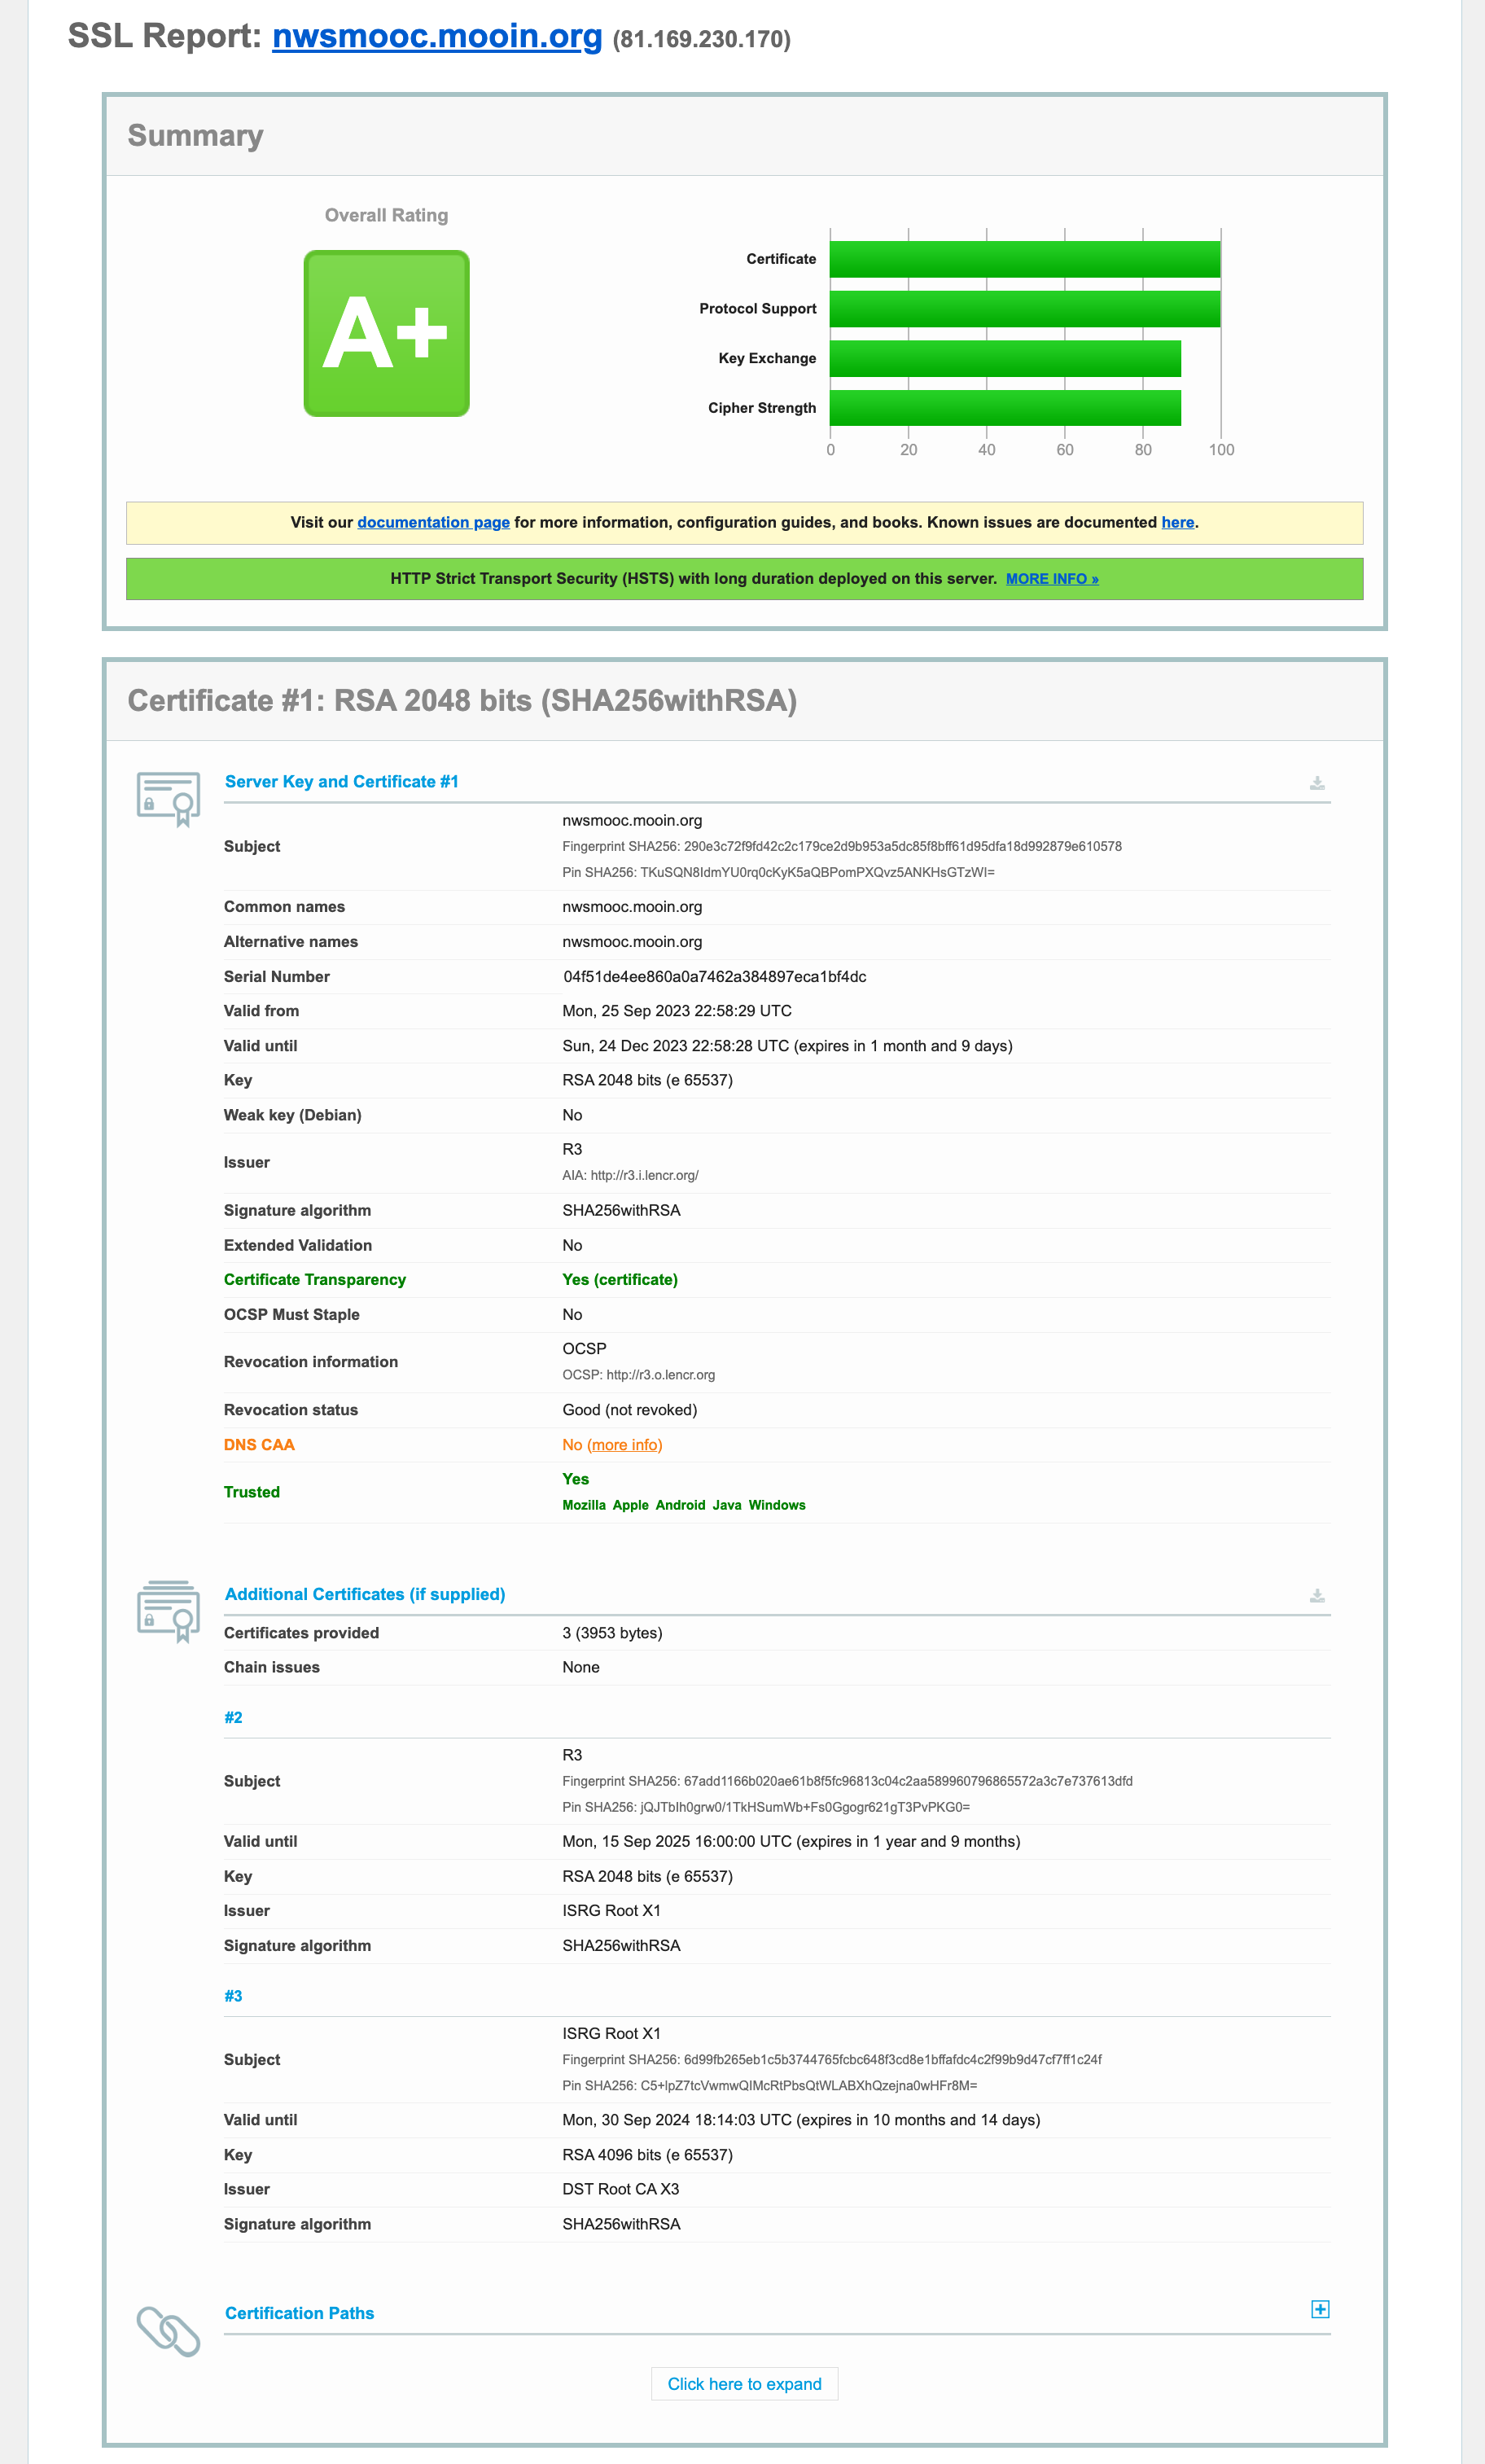
\includegraphics[width=0.75\textwidth]{images/01}
	\centering
	\caption{QualysSSL Test – nwsmooc.mooin.org}
\end{figure}

Der Web-Server hat insgesamt eine A+-Bewertung erhalten und ist dementsprechend auf dem aktuellen Stand / robust was die SSL-Konfiguration angeht.
Das Zertifikat des Servers ist ein 2048-Bit RSA-Zertifikat, das mit SHA256+RSA signiert wurde.
In dem Report von Qualys sind einige wichtige Eckdaten über das Zertifikat des Servers enthalten:

\begin{itemize}
    \item Gültigkeit: Von 25. September 2023 bis zum 24. Dezember 2023
    \item Aussteller: R3
    \item Status: Das Zertifikat wurde nicht widerrufen.
    \item Vertrauenswürdigkeit: Ja – Mozilla, Apple, Android, Java und Windows vertrauen diesem Zertifikat.
\end{itemize}

Außerdem gibt der Bericht die Zertifikate weiter oben in der Zertifikats-Kette an:

\begin{itemize}
    \item Zertifikat \#2: Aussteller R3, RSA 2048 Bit, gültig bis 15. September 2025.
    \item Zertifikat \#3: Aussteller ISRG Root X1, RSA 4096 Bit, gültig bis 30. September 2024.
\end{itemize}

\vspace{0.5em}

---

\begin{figure}[H]
	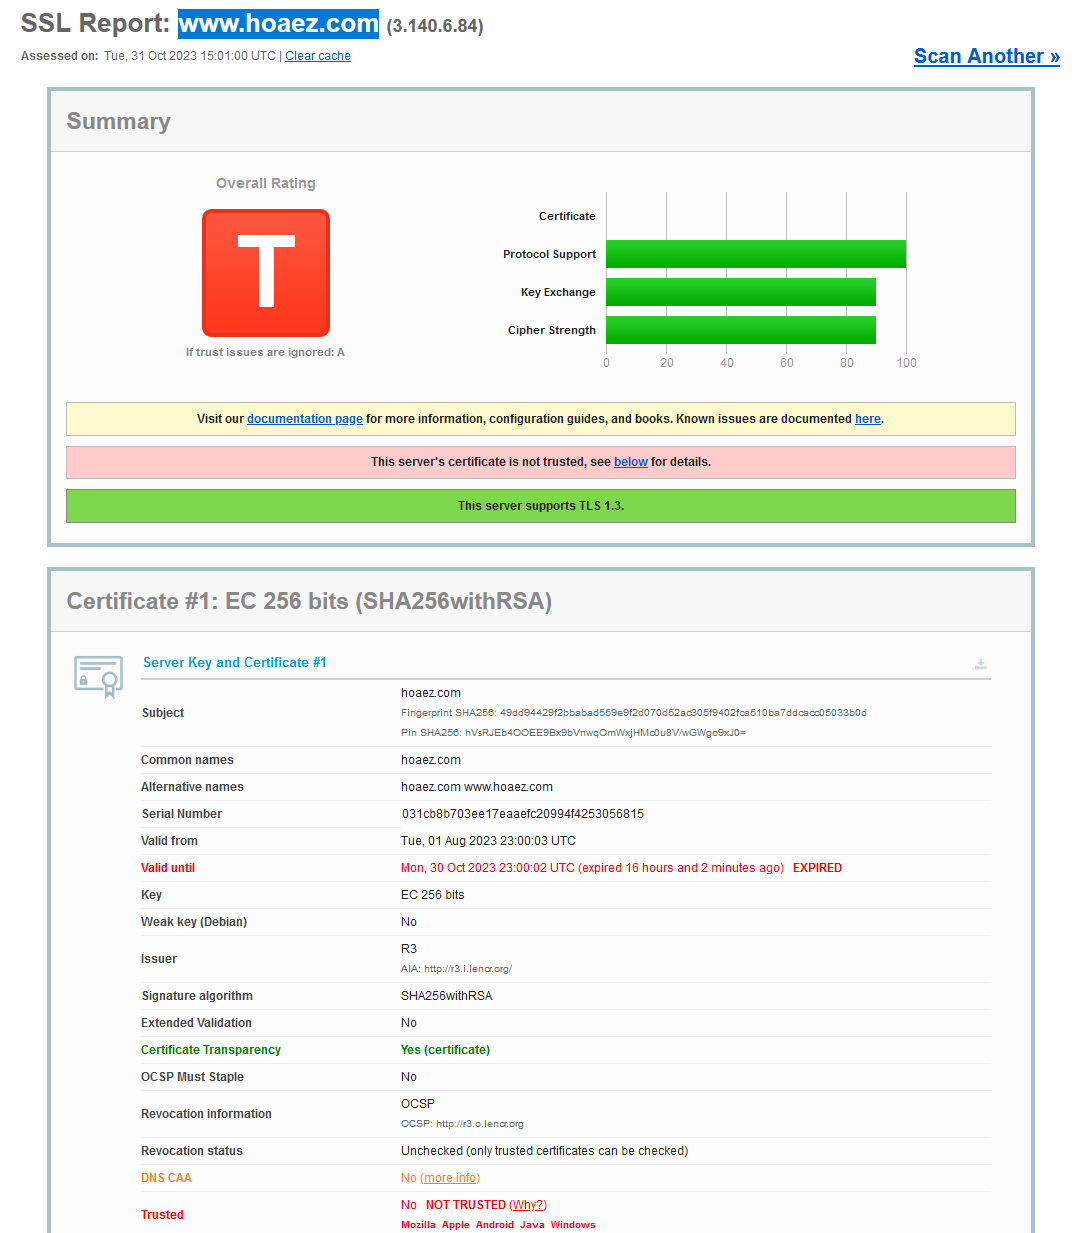
\includegraphics[width=0.75\textwidth]{images/02}
	\centering
	\caption{QualysSSL Test – Recent Worst}
\end{figure}

Der Server www.hoaez.com hat lediglich eine Gesamtbewertung von T erhalten, was bedeutet, dass dem Zertifikat
des Servers nicht vertraut werden kann (e.g. da es abgelaufen ist, oder durch eine Misskonfiguration). Um dennoch einen
Report erstellen zu können, hat Qualys die Vertrauenswürdigkeit bis auf weiteres ignoriert.


Unter der Zusammenfassung gibt es einen Abschnitt, der Details zum Zertifikat des Servers liefert. Diese deuten
explizit darauf hin, dass das Zertifikat (zum Test-Zeitpunkt seit 16 Stunden) abgelaufen und somit nicht mehr gültig ist.
Es ist anzunehmen, dass durch eine Erneuerung des Zertifikates, alle Probleme behoben werden können und der Server wieder
eine ausreichend gute Bewertung erhalten würde.

Das Zertifikat an sich ist verwendet Elliptic-Curve mit 256 Bits und wurde ebenfalls mit SHA256+RSA signiert.

Dieser Report ist ein gutes Beispiel dafür, als Administrator im Idealfall auf sich-selbsterneuernde Zertifikate zu setzen,
um einem Vertrauensverlust der Nutzer (durch eine Warnmeldung des Browsers) entgegen zu wirken.

\newpage

\subsection{SSL Test II}

\subsubsection*{Aufgabenstellung}

Führen Sie den Client-Test von Qualys aus und erklären Sie die Ergebnisse. (Siehe \url{https://clienttest.ssllabs.com:8443/ssltest/viewMyClient.html})

\subsubsection*{Antwort}

Wir haben den Client-Test mit der Mozilla Firefox Version 119.0.1 durchgeführt und folgendes Ergebnis erhalten:

\begin{figure}[H]
	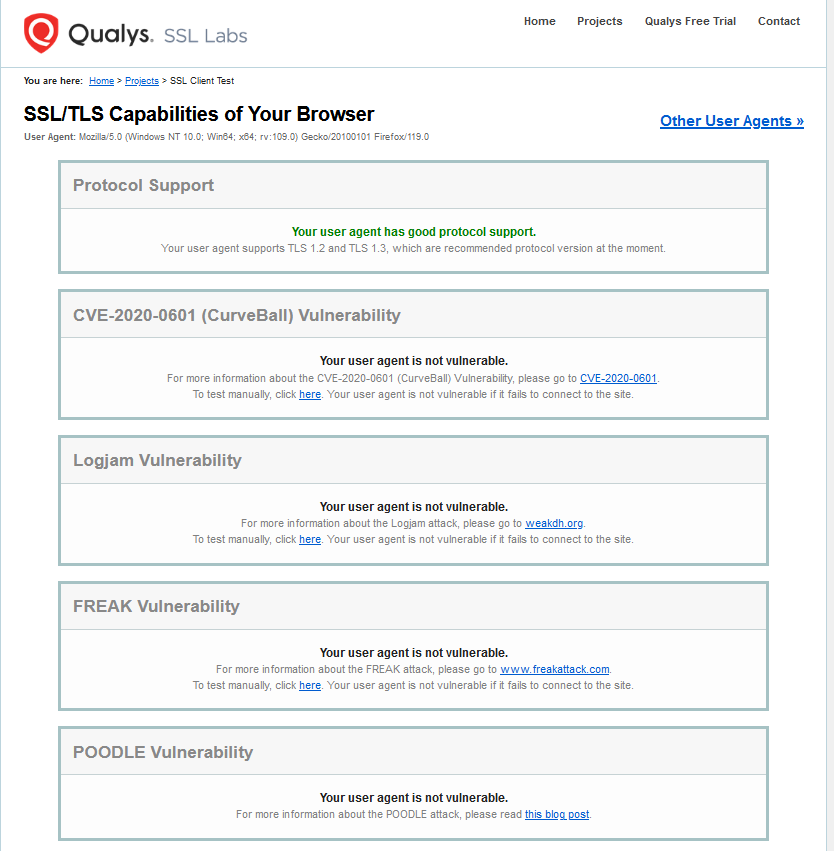
\includegraphics[width=0.75\textwidth]{images/03}
	\centering
	\caption{QualysSSL Test – Browser Capabilities}
\end{figure}

Im Kopf der Ergebnisseite wird eine Zusammenfassung der Bewertung ausgegeben. Es wird zunächst 
die Protokoll-Unterstützung mit grün/gut bewertet – in unserem Fall ob TLS 1.2 und TLS 1.3 unterstützt wird.
Danach folgen spezifische Schwachstellentests:

\begin{itemize}
    \item \textbf{Curveball / CVE-2020-0601} - Schwachstelle im Windows-OS bei der
    	Validierung von digitalen Zertifikaten die potentiell angreifbar für MitM macht.
    \item \textbf{Logjam} - Sicherheitslücke im Diffie-Hellman-Schlüsselaustausch,
		welcher bei verschlüsselten Verbindungen wie TLS verwendet wird. Ermöglicht den Schlüsselaustausch
		zu manipulieren und verschlüsselte Verbindungen zu entschlüsseln.
    \item \textbf{FREAK (Factoring RSA Export Keys)} – Sicherheitslücke, die Angreifern
		es ermöglichte Verschlüsselung von HTTPS-Verbindungen zu umgehen.
    \item \textbf{POODLE (Padding Oracle On Downgraded Legacy Encryption)} - Schwachstelle
		in SSLv2/3 die es ermöglichte die Verschlüsselung zu umgehen.
\end{itemize}

Keine der Schwachstellen sind auf unserem Client vorhanden.

\begin{figure}[H]
	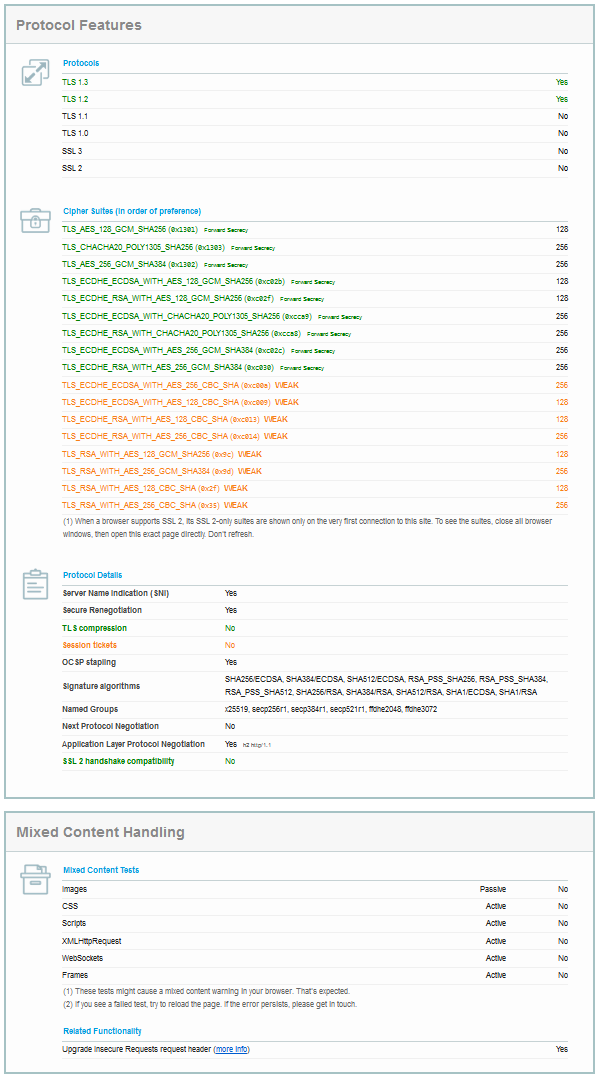
\includegraphics[width=0.75\textwidth]{images/04}
	\centering
	\caption{QualysSSL Test – Browser Protocol Features}
\end{figure}

Es folgt eine Detailauflistung der Protokoll-Features, die ergänzt ist um eine Auflistung der 
unterstützten Cipher Suites in Reihenfolge der Präferenz (von oben nach unten). Dabei werden viele 
kryptographische Verfahren als grün/gut bewertet, einige aber als weak. Dies ist z.B. auf die Duldung 
von SHA (anstatt SHA256) zurückzuführen, oder weil der CBC-Modus (Cipher Block Chaining) erlaubt wird. 
CBC hat bekannte Schwächen, beispielsweise auf Angriffe wie den sogenannten "Padding Oracle Attack".
Die Ermöglichung von CBC in Verbindung mit älteren Authentifizierungsalgorithmen wie SHA1 wird hier 
vermutlich als unsicher (auf englisch: weak) angesehen.

Unter der Überschrift \textbf{Protocol Details} wird als gut/grün hervorgehoben, dass TLS compression 
deaktiviert ist. Dies war ein Feature in älteren TLS-Versionen und sollte Daten komprimieren vor der 
Verschlüsselung, war jedoch angreifbar und wurde daher in Folgeversion deaktiviert. Ebenfalls 
deaktiviert sein sollte die SSL 2 handshake compatibility – dies ist die bereits erwähnte POODLE 
Schwachstelle. Die letzte farbliche Hervorhebung in diesem Abschnitt lautet \textbf{Session tickets – 
No}. Warum die Deaktivierung von Session-Tickets als weak gekennzeichnet wurde, konnten wir nicht 100\% 
feststellen. Der Blog der Betreiber-Webseite beschreibt diesen Eintrag hauptsächlich aus Sicht eines 
Web-Server/-Seiten Betreibers so, „dass session tickets ein alternativer Session-Management Mechanismus 
sei, welcher separate Encryption Keys verwendet, die selten rotiert werden und lieber nicht verwendet 
werden sollten, wenn man die Implementation nicht genau im Detail versteht.“ (vgl.
\url{https://blog.qualys.com/product-tech/2013/06/25/ssl-labs-deploying-forward-secrecy}, abgerufen am 
09.11.2023). Es erschien uns eher als Vorteil denn als Nachteil dass dieses Feature im Firefox 
deaktiviert sei.

Den Abschluss der Ergebnisseite bildet der Abschnitt \textbf{Mixed Content Handling}, in dem die 
Kompatibilität mit diversen Webtechnologien (z.B. CSS, Frames usw.) getestet wird.

\newpage

\subsection{SSL Test III}

\subsubsection*{Aufgabenstellung}

Rufen Sie die Test-Webseiten https://aaacertificateservices.comodoca.com:442/ sowie 
https://aaacertificateservices.comodoca.com:444/  mit Firefox und mit Google 
Chrome auf. Erklären Sie, was passiert. Sind die Resultate bei allen vier Tests so 
wie erwartet?

\subsubsection*{Antwort}

ÜBERARBEITEN

\begin{figure}[H]
	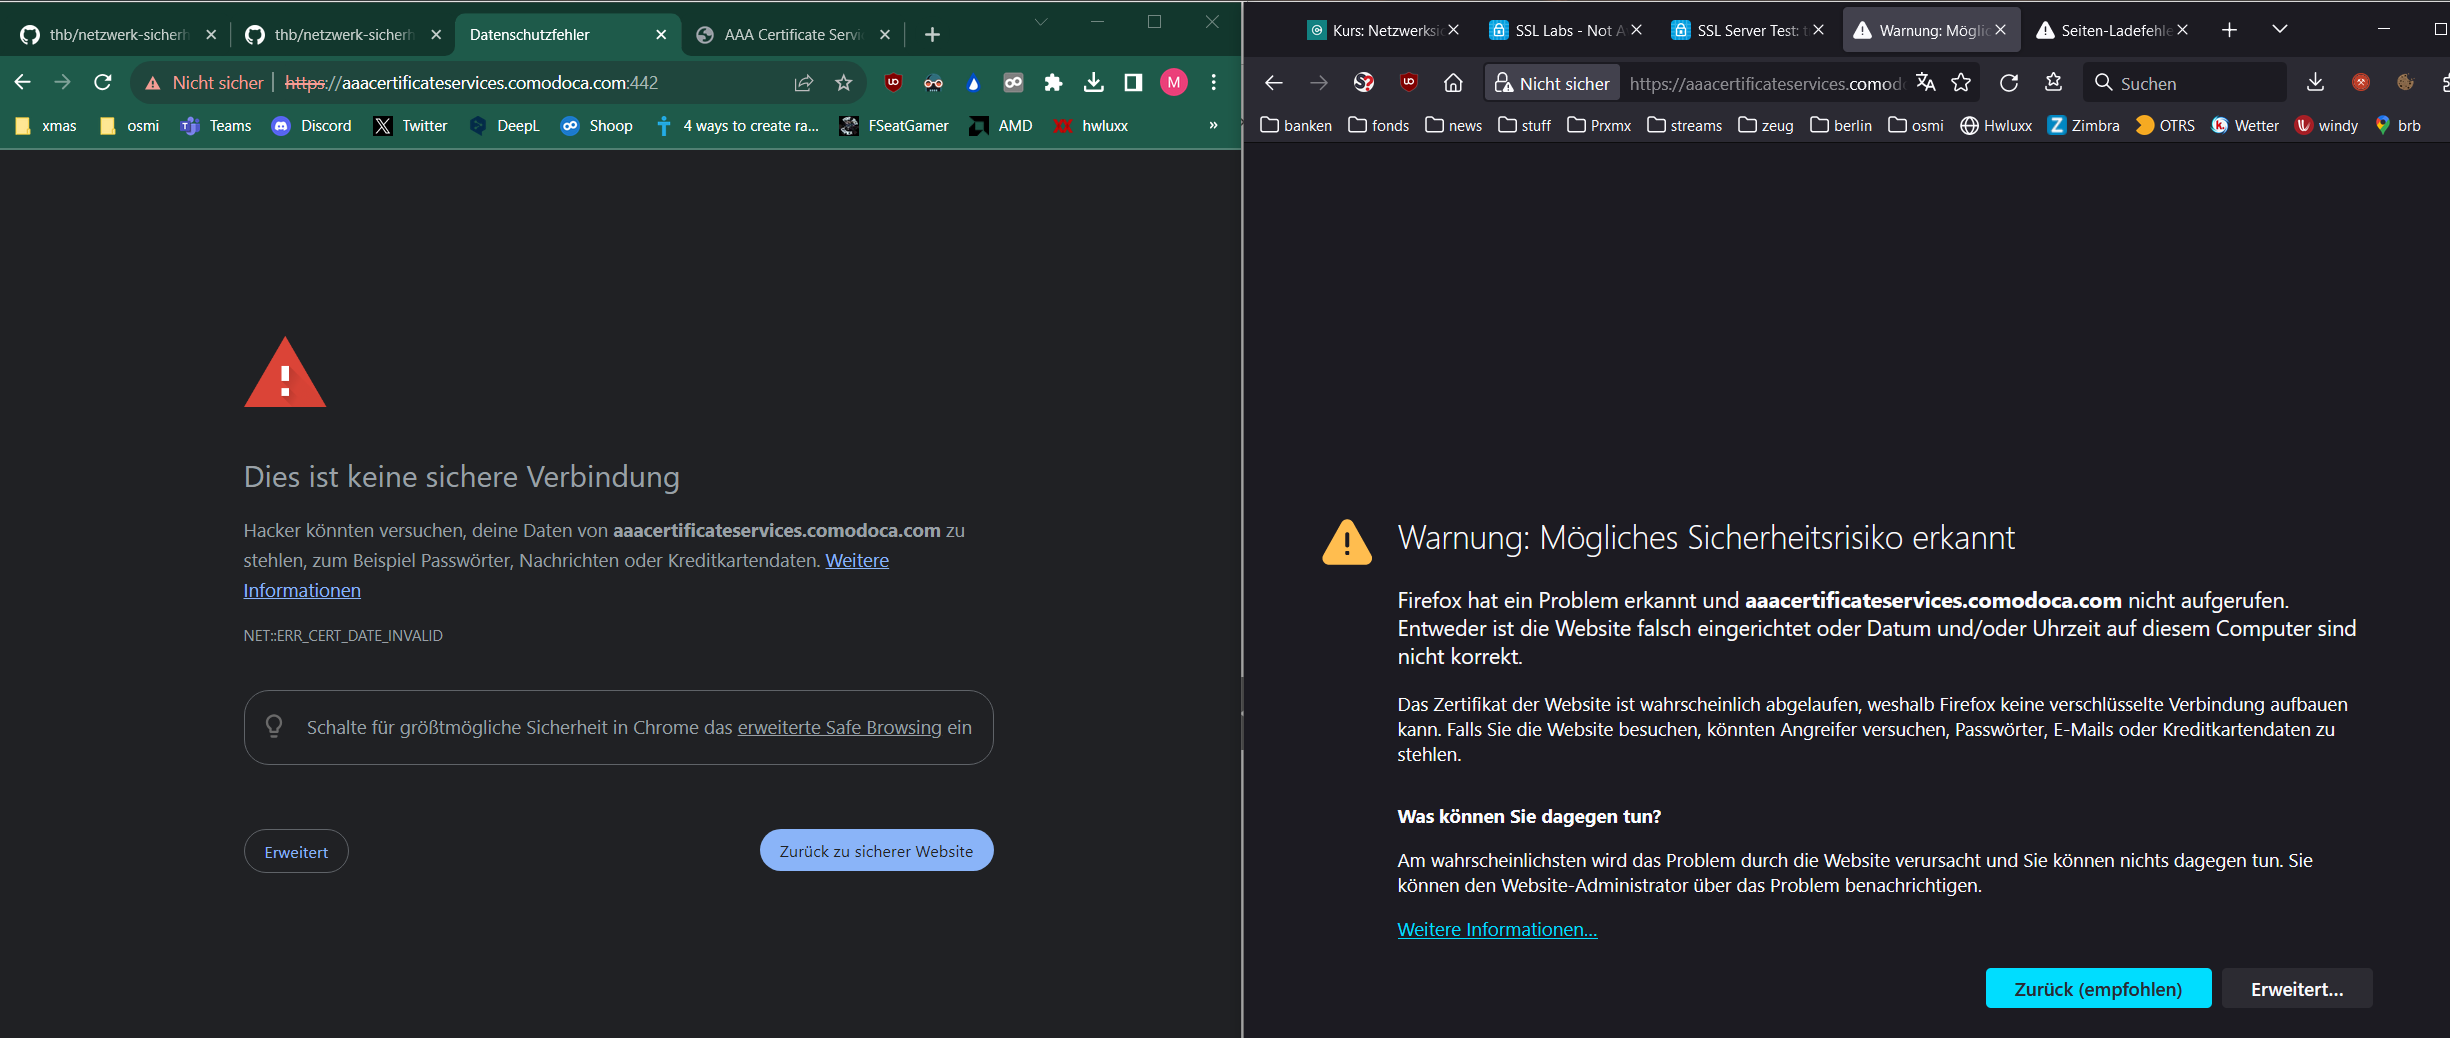
\includegraphics[width=0.75\textwidth]{images/05}
	\centering
	\caption{QualysSSL Test – Browser Protocol Features}
\end{figure}

\textbf{Google Chrome Ergebnisse:}

\begin{itemize}
    \item Der Zugriff auf die Site auf Port 442 führt zu einer Sicherheitswarnung,
		die besagt, dass die Verbindung nicht privat ist.
	\item Der Zugriff auf die Site auf Port 444 zeigt ebenfalls eine Sicherheitswarnung an,
		die darauf hinweist, dass das Sicherheitszertifikat der Site nicht vertrauenswürdig ist.
\end{itemize}

\textbf{Mozilla Firefox Ergebnisse:}

\begin{itemize}
	\item Der Zugriff auf die Site auf Port 442 zeigt eine Warnung vor einem potenziellen Sicherheitsrisiko an.
	\item Der Zugriff auf die Site auf Port 444 zeigt eine Warnung, dass das Sicherheitszertifikat der Site widerrufen wurde.
\end{itemize}

Hinsichtlich der Frage, ob die Ergebnisse wie erwartet sind:

\begin{itemize}
    \item \textbf{Sicherheitswarnungen:} Diese sind zu erwarten, wenn eine Website SSL/TLS-Probleme hat, wie zum Beispiel ein ungültiges, abgelaufenes oder widerrufenes Zertifikat, oder wenn das Zertifikat nicht mit dem Domainnamen übereinstimmt. Es scheint, dass das Zertifikat für die über Port 444 aufgerufene Site widerrufen wurde, was ein kritisches Sicherheitsproblem darstellt, während die Site auf Port 442 ein anderes Zertifikatproblem hat, das die Browser nicht akzeptieren (wie es könnte selbstsigniert, abgelaufen sein oder es könnte eine Hostnamen-Diskrepanz geben).

    \item \textbf{Browser-Konsistenz:} Die Tatsache, dass beide Browser für beide Ports Fehler anzeigen, deutet darauf hin, dass das Problem bei den Zertifikaten der Website liegt und nicht bei den Browsern selbst. Dies ist ein konsistentes und erwartetes Verhalten.

    \item \textbf{Unterschiede in den Browser-Warnungen:} Die Unterschiede in den Sicherheitswarnungen zwischen Chrome und Firefox sind auf die unterschiedlichen Arten zurückzuführen, wie diese Browser Sicherheitsprobleme behandeln und melden. Beide identifizieren jedoch korrekt, dass es ein Problem mit dem SSL/TLS-Zertifikat der Website gibt.
\end{itemize}

Angesichts der Screenshots können wir schlussfolgern, dass die Websites SSL/TLS-Konfigurationsprobleme haben, die dazu führen, dass beide Browser korrekt Sicherheitswarnungen anzeigen. Es wäre ratsam, diese Websites nicht ohne eine sichere Verbindung zu besuchen, da dies sensible Informationen einer Abfanggefahr aussetzen kann. Der Website-Administrator sollte die Zertifikatsprobleme lösen, um einen sicheren Zugang für die Benutzer zu gewährleisten.


Diese Diskrepanz kann aus mehreren Gründen auftreten:

\begin{enumerate}
  \item \textbf{CRL und OCSP}: Chrome und Firefox verwenden möglicherweise unterschiedliche Methoden zur Überprüfung des Widerrufsstatus eines Zertifikats. Chrome überprüft möglicherweise nicht den Widerrufsstatus oder konnte den Certificate Revocation List (CRL) oder Online Certificate Status Protocol (OCSP) Server nicht erreichen. Wenn der Server nicht erreichbar ist, kann Chrome die Verbindung unter bestimmten Bedingungen zulassen.
  \item \textbf{Caching}: Es könnte ein Caching-Problem geben, bei dem Chrome das Zertifikat oder seinen Status zwischengespeichert hat und keinen Live-Check durchführt, um zu sehen, ob das Zertifikat widerrufen wurde.
  \item \textbf{Widerrufsinformationen}: Es ist auch möglich, dass Firefox aktualisierte Widerrufsinformationen hat, die Chrome nicht hat. Dies kann passieren, wenn die Widerrufsinformationen kürzlich aktualisiert wurden und Chrome das Update noch nicht erhalten hat.
  \item \textbf{Browser-Konfiguration}: Die Sicherheitseinstellungen des Browsers könnten unterschiedlich konfiguriert sein. Zum Beispiel könnte Chrome so eingerichtet sein, dass es mit bestimmten Arten von Zertifikatsfehlern fortfährt, die Firefox nicht zulässt, oder umgekehrt.
  \item \textbf{Certificate Pinning}: Chrome könnte das Zertifikat für diese Seite gepinnt haben, was die normale Überprüfung der Vertrauenskette umgehen würde, die sonst zu einer erkannten Widerrufsstatus führen könnte.
  \item \textbf{Software-Versionen}: Wenn ein Browser nicht auf dem neuesten Stand ist, erkennt er möglicherweise neuere Arten von Zertifikaten oder Widerrufsmethoden nicht richtig.
\end{enumerate}

Aus Sicherheitsgründen ist es wichtig, dem restriktiveren Browser in einem solchen Szenario zu vertrauen, in diesem Fall Firefox, der darauf hinweist, dass das Zertifikat widerrufen wurde. Widerrufene Zertifikate deuten darauf hin, dass dem Zertifikat nicht mehr vertraut werden sollte, typischerweise aufgrund eines Kompromisses oder eines Ausstellungsfehlers. Es ist ratsam, das Problem weiter zu untersuchen, möglicherweise indem der Zertifikatsstatus auf anderen Systemen oder Netzwerken überprüft wird, um zu sehen, ob das Problem weiterhin besteht, und die Widerrufsliste der Zertifizierungsstelle zur Bestätigung zu konsultieren.


\newpage

\subsection{Verschlüsselung}

\subsubsection*{Aufgabenstellung}

Installieren Sie VeraCrypt  auf Ihrem Rechner. Hierzu erhalten Sie zusätzlich eine 
VeraCrypt-Datei. In der Datei ist ein normaler und ein versteckter Container 
zu finden, die jeweils eine Datei enthalten. Das Passwort für den normalen 
Container ist der Exponent e des RSA-Schlüssels vom nwsmooc.mooin.org-Server. 
Dokumentieren Sie Ihre Vorgehensweise mit Screenshots und geben Sie 
anschließend das im versteckten Container gefundene Kennwort an.

Hinweis: Zur Bedienung von VeraCrypt können Sie sich beispielsweise hier ein Video 
ansehen: https://youtu.be/atb2pdxd394.

\subsubsection*{Antwort}

ÜBERARBEITEN

Um das zur Verfügung gestellte VeraCrypt File öffnen zu können, soll der Exponent e 
des RSA-Schlüssels der Webseite nwsmooc.mooin.org verwendet werden. Diesen 
Exponenten kann man sich ganz einfach ausgeben lassen, in dem man sich im Mozilla 
Firefox Browser jene Webseite öffnet und auf das Schlosssymbol drückt, um sich 
das Zertifikat anzusehen.

Im Abschnitt „Öffentlicher Schlüssel – Informationen“ bekommt man diesen einfach 
ausgegeben (Siehe Abbildung XXX). Wir merken an dieser Stelle an, dass wir diesen 
Exponenten zunächst auch blind getestet hatten, da in der Praxis fast immer die 
Zahl 65537 als Exponent verwendet wird. Für das RSA Verfahren werden große 
Primzahlen bevorzugt verwendet und der Algorithmus muss dabei unterschiedliche 
Operationen bei der Bearbeitung basierend auf dem Binärcode tätigen. 6553710 ist 
binär kodiert 10000000000000001 (??????????????)
was es zu einer effizienten Zahl für den Algorithmus macht (Einsen werden 
multipliziert, Nullen potenziert).

Mounted man mit VeraCrypt die bereitgestellte Datei und gibt als Passwort 65537 an, 
erhält man Zugriff auf die Datei. (siehe Abbildung XXX)


Der Inhalt des Textfiles „Datei-angezeigter-Container.txt“ lautet:	„Das 
Zugangskennwort für den versteckten Container lautet: 	VerSteCon0815“

Wir konnten uns an das Modul Digitaler Selbstschutz erinnern, in dessen Reportinhalt 
VeraCrypt bereits vorkam, und haben den Container gecloned und ein 2. Mal gemounted, 
wobei wir dieses Mal das Passwort VerSteCon0815 eingegeben haben.

Damit konnten wir Zugriff auf den versteckten Container und seinem Inhalt „Datei-
versteckter-Container.txt“ erhalten.

Der Text dieser Datei lautet:

Das gesuchte Kennwort lautet: HiddenVolumeVeraCrypt

% Die Einstellungen von SilentEye, die Sie für die Fortgeschrittenenaufgabe brauchen, 
% sind:

% Key (für beide Dateien): NWSMOOC_Test
% Passphrase (nur für jpg-Datei): SilentEye_Test

Die anderen Einstellungen entsprechen den Default-Einstellungen

Für mooin.jpg: 
Luminance Interval = 5 
Header Position = bottom
CharSet = UTF8

Für mooin.bmp (Oben beim "Media's encoding format" auf "BMP" wechseln):
Image quality: 96,975% (normal); keine Veränderungen bei "Advanced"
Aktivieren Sie zusätzlich zu "Compressed Data" jeweils auch "Encrypted Data" mit AES256. Dort muss der Key in beide Kästchen eingetragen werden.
Über die SilentEye-Aufgabe erhalten Sie über mooin.bmp übrigens schon vorab eine Aufgabensammlung zur Klausurvorbereitung.


\newpage

\subsection{Steganographie}

\subsubsection*{Aufgabenstellung}

Installieren Sie SilentEye  auf Ihrem Rechner und untersuchen Sie die 
bereitgestellten Beispieldateien. mooin.jpg enthält ein verstecktes Kennwort, 
mooin.bmp eine Datei. Die notwendigen Einstellungen können Sie der Aufgabe mit 
VeraCrypt entnehmen. Dokumentieren Sie Ihre Vorgehensweise mit Screenshots und 
geben Sie das gefundene Kennwort an.

Hinweis: Sollte es Schwierigkeiten geben, wenn Sie beide Dateien nacheinander 
untersuchen, dann schließen Sie SilentEye zwischendurch.

\subsubsection*{Antwort}

ÜBERARBEITEN

SilentEye ist eine Open-Source-Software, die zur Steganographie verwendet wird, um 
zusätzliche Informationen in Bildern und Audiodateien zu verstecken oder auszulesen. 

Um mooin.jpg zu untersuchen, öffnen wir die Datei mit dem Programm Silenteye und 
verwenden die Einstellungen aus der Lösung der Aufgabe 1.4.

Dadurch kann der verborgene Bereich des Bildes erfolgreich entschlüsselt werden und 
gibt als dekodierte Message den Text ``Kennwort: SteganographieInNWSMOOC'' frei.

Mit diesem Kennwort und den bereitgestellten Einstellungen für das zweite Bild, lässt 
sich auch dessen versteckter Inhalt sichtbar machen und entschlüsseln. Wir können an 
dieser Stelle die Datei AufgabensammlungSS16.pdf extrahieren und abspeichern.

\end{document}
